For at hj�lpe med at give et bedre overblik over systemet og hvordan de forskellige lag snakker sammen i forhold til hinanden, vil arkitekturen blive beskrevet her. 

\section{Arkitektur}

Da vi bruger MVC 3 har vi en stor del af vores grundstruktur. MVC som st�r for Model, View, Controll er ogs� delt op i netop disse tre lag. 

\begin{figure}[H]
	\centering
		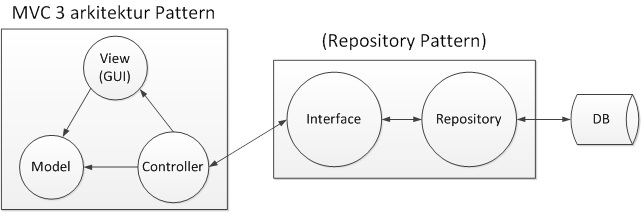
\includegraphics[width=1.00\textwidth]{arkitektur.jpg}
	\caption{Arkitektur}
	\label{fig:arkitektur}
\end{figure}

Som det kan ses p� figur \ref{fig:arkitektur} er MVC kun en del af arkitekturen. Der er implementeret et Repository pattern, for at opn� en r�kke fordele, som vil blive beskrevet i et senere afsnit. MVC controlleren st�r for at skrive til de klasser der er implementeret af repository pattern. Controlleren vil sende et objekt ned til sit repository, som skriver det til databasen. Det skal ses som et data access lag, det er her alt kontakt med databasen starter og stopper. Vores repositories vil hedde CompanyRepository.cs mens interfacet til denne vil hedde ICompanyRepository.cs. Navnet fort�ller selvf�lgelig noget omkring hvilket omr�de dette repository bruges.

P� figur \ref{fig:arkitektur} ses cirkelen kaldet Model. Det er vores klassiske modellag som man ogs� kender det fra 3-lags arkitekturen. Det er i dette lag dom�nemodellen bliver realiseret. Da der bruges Entity Framework styrer dette framework laget for os, og det vil derfor virke tomt. Der benyttes Database First tilgangen til at modellere laget ud fra designet af databasen. Derved bruges Entity Frameworket det meste af tiden til at styre dette lag. Vi laver dog nogle modelklasser manuelt s� som wrapper-klasser, eller ViewModels. Disse kunne blandt andet bruges hvis man vil sende to entity klasser til samme view. Eller har brug for nogle flere properties, som man ikke er interesseret i bliver gemt i databasen. Der vil komme eksempler p� disse senere i rapporten.

View p� figur \ref{fig:arkitektur}, er det grafiske interface, som st�r for at vise den HTML brugeren skal se. Et View benyttes ofte sammen med en model. Det vil sige et objekt med en r�kke properties som man �nsker vist i viewet. Det kunne v�re et Company objekt der bliver sendt som model, hvor efter viewet har adgang til dens properties. Her er ogs� mulighed for at bruge IEnumerables hvis det er lister man vil skrive ud. Hvis man har en web-form p� siden er det muligt at sende samme type objekt tilbage til controlleren, med alle de nye properties man har sat i web-formen. Et view vil ligge en mappe af samme navn som den controller den h�re til. De vil typisk have et navn der forklare indholdet af siden, f.eks. Company.cshtml.

Normalt er det meningen, at view- og modellaget er skarpt adskilt af controllerlaget, s� model og view aldrig kommunikerer direkte. Frameworket er dog skruet s�dan sammen, at controlleren sender et model-objekt direkte til viewet. 

Controller p� figur \ref{fig:arkitektur} er vores controllerlag. Controlleren styrer hvad der sker i applikationen, og st�r for at f� vist de rigtige views. Den vil minde meget om det controllerlag man ogs� ser i 3-lags arkitekturen. Det er her vi modtager input fra brugeren og opretter objekter som vi sender videre ned til vores data access lag. (Repository pattern). Alle controllere hedder Controller til sidst. Alts� en controller til at styre sine companies ville oplagt hedde CompanyController.cs. Dette er bestemt af MVC 3. 

Selve mappe- og filstrukturen bliver selvf�lgelig i h�j grad bestemt af MVC, men for at g�re overblikket af systemet totalt vil vi kort beskrive strukturen her.

\begin{figure}[H]
	\centering
		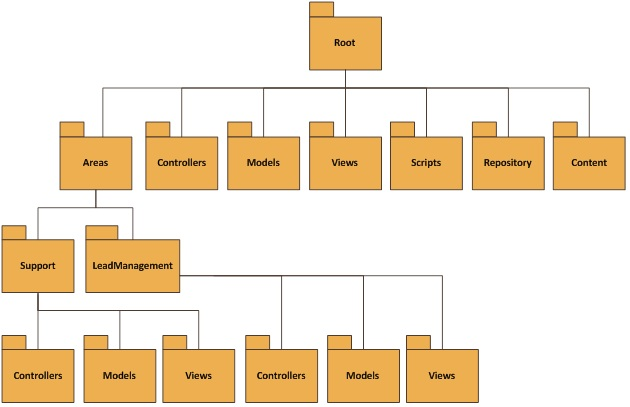
\includegraphics[width=1.00\textwidth]{mappestruktur.jpg}
	\caption{Mappestruktur}
	\label{fig:Mappestruktur}
\end{figure}

I roden af projektet vil man finde nogle config filer med forskellige ops�tninger af sitet. Blandt andet SQL forbindelse. Der udover bruges Content til alle CSS filerne, Scripts til JavaScript og jQuery frameworket. I Repository ligger repository klasserne samt deres interface. Controllers, Models og Views er MVCs struktur, og burde v�re selvforklarende. Mere interessant er Areas \citep[pp. 374-381]{freeman2011pro} som er MVCs m�de at lave sub-directories p�. Hver mappe i et Area f�r nemlig hver sin Controllers, Models og Views mappe som virker p� samme m�de som dem i Root mappen. Det g�r det nemt at flytte en del af systemet ud i et sub-directory, da alt vil opf�re sig p� samme m�de s�fremt det ligger i samme sub-directory.